\section{Gaussian Mixture Model}

Gaussian mixture models make the assumption that data is generated from Gaussians. To be more precise a convex-combination of Gaussian distributions:
$$p(x \; | \; \theta) = p(x \; | \; \mu, \Sigma, w) = \sum_{j=1}^k w_j \cdot \mathcal{N}(x; \mu_j, \Sigma_j)$$

\begin{center}
	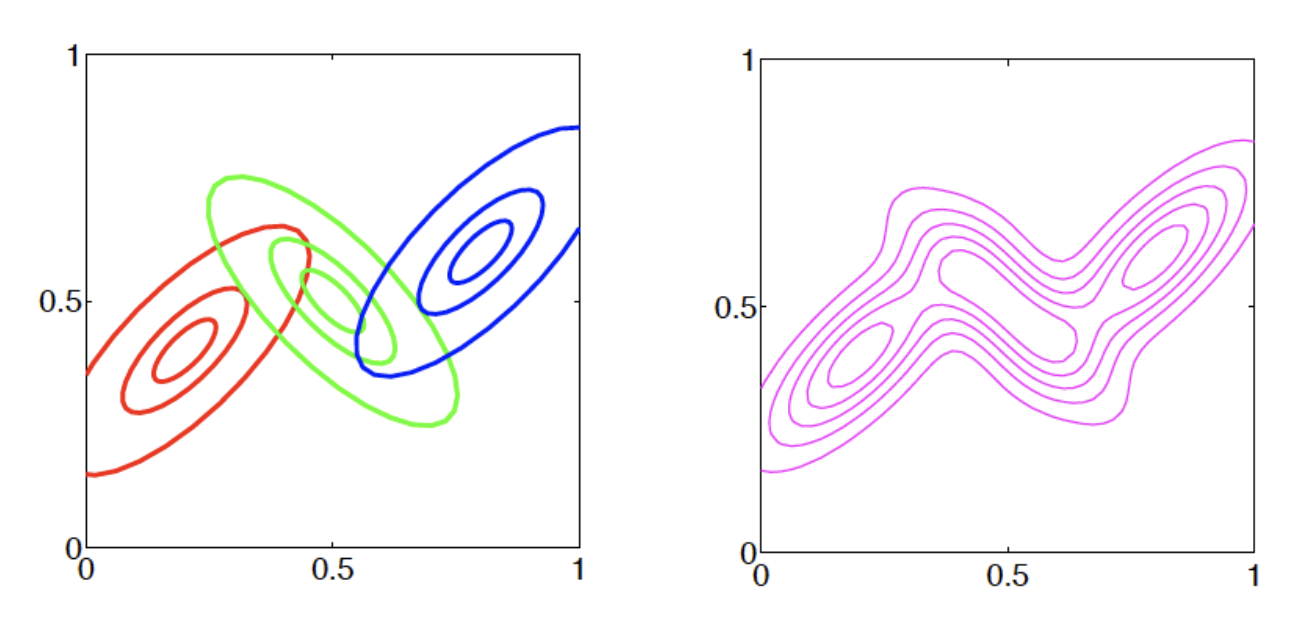
\includegraphics[width=\columnwidth]{gmm.png}
\end{center}

We do not know the labels $z$ for the data and can only see the level-set on the right. The problem we try to solve is to estimate the parameters for the Gaussian distributions (minimize log-likelihood).
$$(w_{i:k}^*, \mu_{i:k}^*, \Sigma_{1:k}^*) = \argmin \; - \sum_{i=1}^n \log \sum_{j=1}^k w_j \cdot \mathcal{N}(x_i \; | \; \mu_j, \Sigma_j)$$

This is a nonconvex objective, but we can still try to apply SGD. But there is a better way to fit this model. The idea is that fitting a GMM is similar to training a GBC without labels. We want to apply an iterative approach where we first start with some guess for our parameters, predict the unknown labels and then impute the missing data. Now we can get a closed form update for our model which we then use to refine our parameters.

\subsection{Hard-EM Algorithm}

First we are gonna look at the simpler version of the EM (expectation maximization) algorithm:
\begin{itemize}
	\item Initialize the parameters $\theta^{(0)}$
	\item For $t = 1,2,...$ :
		\begin{itemize}
			\item \textbf{E-Step}: predict the most likely class for each data point:
				\begin{align*}
					z_i^{(t)} &= \argmax{z} \; p(z \; | \; x_i, \theta^{(t-1)}) \\
					&= \argmax{z} \; p(z \; | \; \theta^{(t-1)}) \cdot p(x_i \; | \; z, \theta^{(t-1)}))
				\end{align*}
			\item \textbf{M-Step}: compute MLE of $\theta^{(0)}$ as for GBC
		\end{itemize}
\end{itemize}

There are some problems with this approach, for one points are assigned a label even though the model is uncertain. Further it tries to extract too much information from a single point. In practice, this may work poorly if clusters are overlapping.

\subsection{Soft-EM Algorithm}

Instead of predicting hard class assignments for each data point we want to predict class probabilities. 
\begin{itemize}
	\item Initialize the parameters $\theta^{(0)}$
	\item For $t = 1,2,...$ :
		\begin{itemize}
			\item \textbf{E-Step}: calculate the cluster membership weights for each point:
				\begin{align*}
					\gamma_j^{(t)}(x_i) &= p(z_i = j \; | \; x_i, \theta_j^{(t-1)}) \\
					&= \frac{w_j \cdot p(x_i ; \theta_j^{(t-1)})}{\sum_k w_k \cdot p(x_i ; \theta_k^{(t-1)})}
				\end{align*}
			\item \textbf{M-Step}: compute MLE with closed form solution:
				\begin{align*}
			 		w_j^{(t)} &= \frac{1}{n} \sum_{i=1}^n \gamma_j^{(t)}(x_i) \quad \; \mu_j^{(t)} = \frac{\sum_{i=1}^n x_i \cdot \gamma_j^{(t)}(x_i)}{\sum_{i=1}^n \gamma_j^{(t)}(x_i)} \\
			 		\Sigma_j^{(t)} &= \frac{\sum_{i=1}^n \gamma_j^{(t)}(x_i)(x_i - \mu_j^{(t)})(x_i - \mu_j^{(t)})^\top}{\sum_{i=1}^n \gamma_j^{(t)}(x_i)}
			 	\end{align*}
		\end{itemize}
\end{itemize}


